\documentclass{article}

\usepackage{blindtext}
\usepackage{amsmath}
\usepackage{graphicx}
\usepackage{subcaption}
\usepackage{float}
\usepackage[ruled,vlined]{algorithm2e}
\usepackage{hyperref}

\bibliographystyle{unsrt}

\usepackage{booktabs}
\usepackage{array}
\usepackage{longtable}



\begin{document}

\title{A bio-inspired minimal model for non-stationary K-armed bandits}
\author{Krubeal Danieli, Mikkel Elle Lepperød}

\maketitle

\newpage

\tableofcontents

\newpage


\section{Introduction}
\hfill \break
\vspace {0.5cm}

% brief introduction to decision making and the brain.
The ability to make decisions for long-term reward maximization is a fundamental aspect of cognition. The brain is has evolved specialized and interconnected regions to implement this behaviour under the constraints of biology.
The Pre-Frontal Cortex (PFC) is considered a fundamental high-level region for attention and cognitive control, in particular the medial PFC \cite{millerIntegrativeTheoryPrefrontal2001a, sheynikhovichLongtermMemorySynaptic2023}.
The orbitofrontal cortex (OFC) is thought to be involved in motivation and representation of the expected value of the actions, either positive or negative \cite{odohertyAbstractRewardPunishment2001, ricebergRewardStabilityDetermines2012, tremblayRelativeRewardPreference1999}, action selection in uncertain environments \cite{elliottDissociableFunctionsMedial2000}, and contextual processing \cite{frankAnatomyDecisionStriatoorbitofrontal2006}.

% bridge between decision making and the k-armed bandit problem.
Concerning decision-making, simple and well-studied ecological settings are foraging tasks, such as food search. In this problems, the agent is usually asked to choose between different options to maximize an expected reward.
In nature, animals have been shown to exhibit different strategies depending on context.
\textit{Matching behaviour} is a well-known phenomenon in which the animal's decision patterns are proportional to the reward probability of the available options.
Such behaviour is thought to result from the trade-off between exploration and exploitation \cite{suttonReinforcementLearningProblem1998, nivEvolutionReinforcementLearning2002}.
In fact, this is a well known phenomenon in the reinforcement learning literature, in which an agent is faced with the dilemma of exploring new alternatives, potentially more rewarding, or exploiting known options, despite being possibly sup-optimal.
A popular formalization of these type of tasks is the \textit{multi-armed bandit problem} (MABP) \cite{averbeckTheoryChoiceBandit2015}. This settins is usually described in terms of a slot machine endowed with $K$ distinct levers, also called arms.
During a round, the agent selects one of the levers and collects a reward $R$ according to an unknown reward probability specific to the chosen lever.
The goal is simply to maximizes the total reward after a given number steps, which is achieved by effectively updating a selection policy after each round.
This problem has been extensively studied in the context of reinforcement learning, and it is considered a fundamental building block for more complex tasks \cite{suttonReinforcementLearningProblem1998}.

% brief introduction of the k-armed bandit problem and previous algorithms.
% \subsection{Related work}
\hfill \break
% overview of the main solutions proposed in the literature from a computational perspective.
There exists various flavours of this problem, with the simplest having a stationary reward distribution.
Over the years, several algorithms have been proposed, alongside with their theoretical guarantees.
In this regard, Thompson sampling is a popular algorithm that has been shown to achieve near-optimal regret bounds in the stochastic setting \cite{agrawalAnalysisThompsonSampling2012, kaufmannThompsonSamplingAsymptotically2012}.
This approach relies on Bayesian optimization, where the goal is to maintain a posterior distribution over the reward probabilities of the actions, and selecting actions accordingly.
Another popular algorithm is Upper Confidence Bound (UCB), which has been shown to achieve near-optimal regret bounds in the adversarial setting \cite{auerFinitetimeAnalysisMultiarmed2002}.
The approach is based on the idea of maintaining an upper limit on the reward probabilities of the actions, and selecting actions accordingly.
Other successful algorithms are $\epsilon$-greedy and VDBE \cite{gittinsBanditProcessesDynamic1979, banMultifacetContextualBandits2021, tokicAdaptiveEGreedyExploration2010, tokicValueDifferenceBasedExploration2011}.
% outline of lack of bio-realism and what we currently know about how the brain might solve this task.
Nonetheless, despite their success they have little resemblance to neural dynamics nor clear functional similarity to brain regions.

% aim of the work
In this work, we propose a biologically plausible algorithm using rate neurons applied to stochastic bandit problems, more challenging variants of the original task endowed with \textit{concept drift}, where the reward distribution changes over time \cite{garivierUpperConfidenceBoundPolicies2008, besbesStochasticMultiArmedBanditProblem2014, cavenaghiNonStationaryMultiArmed2021}.
% brief overview of the model
The architecture of our model consists of two connected neuronal layers, both with as many neurons as the arms of the bandit task.
The first layer is inspired by the functionality of the OFC, and its scope is to maintain an active representation of the arms weighted by the input from the second layer.
The second, modeled after the ACC, is meant to represent the value of the arms, and its input connections are updated through a learning rule dependant on the reward history and current connectivity pattern.

% main motivations
Our model features two important aspects of the brain during decision making. Firstly, the option selection process itself is implemented as a dynamical interaction between neural populations, similarly to bump attractor networks for perceptual cognition \cite{carrollEncodingCertaintyBump2014, esnaola-acebesBumpAttractorDynamics2021}.
The final choice of the arm is achieved by the agreement or disagreement between the two populations, and it depends on their underlying value representation \cite{bariDynamicDecisionMaking2021, houstonMatchingBehavioursRewards2021}.
Secondly, plasticity is based on a non-associative learning rule, endowed with a non-linear kernel for the weight update term.
% The specific values of a parametrization of the kernel has been optimized through an evolutionary algorithm.
Behind this design choice there is our hypothesis that the scale of the synaptic update should vary non-linearly according to its magnitude.
This consideration is aligned with the idea that the learning rate is a parameter specific to each neuron, and that it can change according to some policy or inductive bias.
This approach has been already adopted in several computational architectures, for instance in spiking neural networks \cite{inglisModulationDopamineAdaptive2021} and for synaptic metaplasticity \cite{iigayaAdaptiveLearningDecisionmaking2016}.
Lastly, there is experimental evidence that this adaptation function might be covered by dopamine \cite{toblerAdaptiveCodingReward2005}.
Indeed, its involvement in calculating prediction errors and reward signaling is well established \cite{schultzNeuralSubstratePrediction1997}, as well with its modulation of  high-level cortical networks like the PFC \cite{didomenicoDopaminergicModulationPrefrontal2023, lohaniDopamineModulationPrefrontal2019, dardenneRolePrefrontalCortex2012}.


% \newpage



\section{Methods}

% brief outline of the section
\noindent The following section is organized as follows. First, we introduce a formalization of general problem setting, together with the variants considered in this work. Then, we outline the architecture of our model and how it can be mapped to neurobiology. Finally, we describe the learning procedure,
and showcase its dynamics in a simple example.


% mathematical formulation of the k-armed bandit problem.
\subsection{Binomial K-armed bandit problem}
\hfill \break
\noindent The standard formulation of the task is structured as a set of $K$ arms (or levers) $\mathcal{A}_{K}=\{a_{1}\ldots a_{K}\}$, with an associated reward distribution $\mathbf{p}=\{p_{1}, \ldots p_{K}\}$.
At each iteration, the agent pulls an arm and collects a possible reward drawn as a Bernoulli variable $R\sim \mathcal{B}(\{0,1\},p_{k})$. The agent's objective is maximizing the total reward $\sum^{T}_{t} R_{t}$, after a certain number $T$ of rounds, also called horizon.
Importantly, the agent is unaware of the true reward probabilities, and thus has to make its decisions following a certain policy, denoted as $\pi$.
In the reinforcement learning literature, the policy is often defined as a distribution over actions, here the arms $\mathcal{A}_{K}$, given the current state at time $t$. In the bandit problem, the state can be taken to correspond to the history $h_{t}$ of past actions and rewards in the period
$(0\ldots t]$, and the policy as a function that return a selected arm $\pi(h_{t})=a_{t}$ \cite{qiForcedExplorationBandit2023}.

Given the inherent stochasticity of the feedbacks from the environment, the policy is affected by the so-called exploration-exploitation trade-off, which here is phrased as the contrast between the option of the arm with the estimated highest expected reward versus the option to explore other arms, so to gather more information.
A common approach is the $\epsilon-$greedy policy, where the choice to explore is selected with a probability $\epsilon$.
Moreover, it is often preferable to have a more explorative behaviour early during the training, with the intent to have a good sample size for the empirical reward distribution, which can be later exploited for maximizing reward.

% regret
Another important concept in multi-armed bandit problems is \textit{regret}. Intuitively, it is defined as the deviation of the total reward obtained by the agent from the optimal reward that could have been obtained by always choosing the arm with the highest expected reward.
Formally, for a stationary distribution\footnote{\textbf{<<NB>>} should I generalize to non-stationary distribution, e.g. using extected values?} the regret is defined as:
\begin{equation}
    \rho=R^{*} - \sum^{T}_{t} R_{t}
\end{equation}

\noindent where $R^{*}$ is the reward obtained by always choosing the arm $a_{k}$ associated with the highest expected reward: $R^{*}=T\max_{k}\{\mathbf{p}\}$, and $R_{t}$ is the empirical reward obtained up to time $t$ by following policy $\pi$: $R_{t}=\sum^{T}_{t=1}\mathcal{B}(\pi(h_{t}))$.
The regret is a measure of the performance of the agent, and it is often used to compare different algorithms. The goal of the agent is to minimize the regret, and thus maximize the total reward.

% minimal model description

\subsection{Model description}
The model is constructed as a rate network of two populations of neurons \textit{M} and \textit{P}, the former representing the memory trace of the \textit{K} available options (\textit{i.e.} the bandits), and the latter representing the value of the options under the current policy.
More formally, the model is described by a set of coupled ordinary differential equations (ODEs) that capture the decision-making process in two distinct neural spaces.
The first equation tracks the evolution of the neural activity $\textbf{u}$ of \textit{M}, while the second tracks the activity $\textbf{v}$ of the \textit{P}. The time constants $\tau$ are the same for both equations and are set to $\tau = 10$ ms.


\begin{equation}
\begin{aligned}
    \tau \dot{\textbf{u}}&= -\textbf{u} + \textbf{v} + \textbf{I}_{\text{ext}} \\
    \tau \dot{\textbf{v}}&= -\textbf{v} + \textbf{z} \odot\textbf{u}
\end{aligned}
\end{equation}

\noindent The external input $\textbf{I}_{\text{ext}}$ is a constant input that is used to set the initial conditions of the neural activity $\textbf{u}$.
The term $\textbf{z}$ is a vector that weights the contribution of the active options $\textbf{u}$ to the value representation $\textbf{v}$, and functionally it is the core of the policy adopted by the model.
In practice, $\textbf{z}$ defined as a function of the synaptic weights $\textbf{W}^{MP}$ from \textit{M} to \textit{P} as $\textbf{z} = \Phi_v(\textbf{W}^{MP})$. Importantly, the connections are not fully connected, but rather are simply one-to-one mapping between the corresponding neurons in each
population, such that the weight matrix $\textbf{W}^{MP}$ is simply a matrix $K\times 1$, namely a vector.
The function $\Phi_v$ is a chosen to be a sum of a generalized sigmoid and a Gaussian, whose contributions are weighted by a parameter $r$:

\begin{equation*}
    \Phi_v(x) = r\gamma_{1} \frac{1}{1 + e^{-\beta(x-\alpha)}} + (1-r)\gamma_{2} \exp\left(-\frac{(x-\mu)^2}{2\sigma^2}\right)
\end{equation*}

\noindent The motivation behind this choice is to express a function that possesses a bounded region (depending on $\mu,\,\sigma$) at a high/low peak (depeding on the value of $\gamma_{2}$), and a continuous transition to a constant value (depending on the steepness of the sigmoid $\beta$, shift
$\alpha$, and intensity $\gamma_{1}$).

\hfill \break
\textbf{Option selection} \\
The decision-making process within a single round is structured in two distinct phases. Initially, the model receives a constant external input targeting all neurons in the memory population \textit{M} equally.
During this phase, $I_{\text{ext}}$ works as an equilibrium value while the reciprocal interactions with population \textit{P} push $\textbf{u}$ to different values, depending on the current policy encoded in $\textbf{z}$. However, in the early rounds the weights $\textbf{W}^{MP}$ are zero, and thus
the contribution from \textit{P} is null. After a fixed amount of time $\sim 5 \text{s}$, the second phase begins. Here, the external input is removed and the model is left to evolve autonomously, and since there are no recurrent connections in neither population the dynamics is entirely driven by their coupling. \\
A selection $\hat{k}$ is sampled after another fixed amount of time $\sim 5 \text{s}$, and it is defined according to the following rule:

\begin{equation*}
    \hat{k} =
    \left\{
        \begin{array}{ll}
            \text{argmax}_{k}\{\textbf{v}\} & \text{\textit{if}}\; \text{argmax}_{k} \{\textbf{v}\} = \text{argmax}_{k} \{\textbf{u}\} \\
            \text{random}(K) & \text{\textit{otherwise}}
        \end{array}
    \right.
\end{equation*}

\noindent The selection rule is simple: if the value representation $\textbf{v}$ is in agreement with the memory trace $\textbf{u}$, then the option with the highest value is selected. Otherwise, a random option is chosen. This rule is a way to express the exploration-exploitation trade-off, and it is dependent on the current policy $\textbf{z}$.

\hfill \break
\textbf{Learning} \\
Given a selected option, the environment (bandit) samples and returns a reward $R\in [0, 1]$.
Then, the connections $\textbf{W}^{MP}$ for the neuron corresponding to the option $k$ are updated according to the following plasticity rule:

\begin{equation}
    \Delta \textbf{W}^{MP}_{k} = \tilde{\eta}_{k} \left(R\cdot W^{+}- \textbf{W}^{MP}_{k}\right)
\end{equation}

\noindent
Where $W^{+}$ is a constant value that sets the upper bound for the synaptic weights, and it is set to $W^{+} = 5$, while $\tilde{\eta}_{k}$ is the learning rate for the option $k$ determined by a function of the current weights $\textbf{W}^{MP}_{k}$ and its shape is the same as $\Phi_{v}$, but with
different parameters.




% Evolution: fitness evolution
\subsection{Evolution search}
The optimization of the hyper-parameters was performed using the Covariance Matrix Adaptation evolutionary strategy algorithm (CMA-ES) \cite{igelCovarianceMatrixAdaptation2007}.
The search was run with a population of $256$ individuals (unique set of genomes corresponding to a sample in parameter space) for $40$ generations. The fitness function was defined as the average reward obtained by an individual over 2 independent iterations.
The results are summarized below in figure \ref{fig:evolution}.

\begin{figure}[H]
    \centering
    \includegraphics[width=1.0\textwidth]{figures/evolution_plot.png}
    \caption{\textsc{Evolution of the model over generations.} - Left: \textit{top fitness, mean and standard deviation (16-84 percentile) of the population over generations.} - Top-Right: \textit{option value and learning rate Gaussian sigmoid functions parametrized according to the genome of the fittest individual}
    Bottom-Right: \textit{activation function for population $v$ and $u$}}
    \label{fig:evolution}
\end{figure}

% comment on the evolved functions
\noindent The evolution results show a steady improvement of the fitness over generations, before hitting a plateau corresponding to the theoretical optimal ($\sim 0.9$) of the chosen simulations.

\textbf{TELL ME ABOUT THE RESPONSE FUNCTIONS, LIKE IS IT A TYPE II NEURON FR?} Regarding the evolved functions, the option value function $\Phi_{v}$ is characterized by a steep sigmoid curve, with a marked.
This is consistent with the idea that the input of population $U$ to population $V$ is weighted maximally for high option values (strong synapses), whereas for weaker estimates the contributions are low or close to zero, allowing for more exploration.

The learning rate function $\Phi_{\eta}$ is instead characterized by a marked bell-shaped curve, given a parameter $r=0.06$. The associated Gaussian has a positive mean located at $\mu=1.$, which aligns approximately with the local valley of the weight function $\Phi_{v}$.
A possible interpretation is that it serves as a mechanism to ensure that the learning rate is high when the value options are more uncertain, and low otherwise, thus preventing overshooting and oscillations in the weight updates.
This adaptive behaviour is in line with known neuronal dynamics such as homeostatic plasticity, which works towards a stabilization of synapses, for instance through synaptic scaling and proportional updates \cite{citriSynapticPlasticityMultiple2008}.
A variable learning rate is an important feature of several plasticity rules, from the more biologically plausible like the Oja \cite{ojaOjaLearningRule2008} to deep learning optimizers like Adam \cite{kingmaAdamMethodStochastic2017}.


\subsection{Bio-inspired features}

The model is inspired by the functioning of the prefrontal cortex (PFC) and its importance in decision-making processes. In particular, the two population $U, V$ of the model can be related to the orbito-frontal cortex (OFC) and anterior cingulate cortex (ACC), respectively.
More specifically, the OFC is known to be involved in the representation of the state different options and update their value with respect to rewarding outcomes and their history \cite{lukChoiceCodingFrontal2013, kennerleyDecisionMakingReward2011a}.
The ACC has been associated to action values and influencing the exploration-exploitation assessment \cite{khamassiChapter22Medial2013}. Further, its dynamic interplay with the OFC is observed to elicit transient pre-stimulus activation, which biases the decision towards the most valuable option \cite{funahashiPrefrontalContributionDecisionMaking2017, marcosDeterminingMonkeyFree2016, balewskiValueDynamicsAffect2023}.

In the model, the first layer represents the available options, while the learned connections with the second layer encode their values based on the recent reward history.
Another similarity with this particular pre-frontal circuit is the realization of a choice as a sample of the network state after a period of autonomous neural activity, where the stability of the neural activations depend on the strength and reliability of the highest option value \cite{backmanEffectsWorkingMemoryTraining2011, enelStableDynamicRepresentations2020}.
Moreover, the application of the function $\Phi_{v}$ on the connections $\textbf{W}^{UV}$ can be regarded as meta-plasticity, mediated by a neuromodulator \cite{wangMetalearningNaturalArtificial2021}.




%\newpage


\section{Results}

The model has been applied to two non-stationary environments.

\subsection{Zero-steps distribution shift}
In this first setting, as the end of a trial $i$ the arm distribution changes immediately to a new one $i+1$ as $\mathbf{\pi}_{i} \to \mathbf{\pi}_{i+1}$.

\begin{figure}[h]
    \centering
    \includegraphics[width=0.65\textwidth]{figures/drawing.png}
    \caption{\textsc{Performance with variable number of arms} - \textit{each plot is an average of 50 simulations with K numbers of arms, the x-axis are rounds, the central vertical line signals the start of the second trial, the y-axis is the reward fraction.
            The shaded area is the reasonable reward
    range, where the lower bound is the chance level and the upper bound the best reward (following the optimal policy). The model performance is in red, while Upper-Confidence Bound green, Thompson Sampling blue, and Epsilon-Greedy orange. }}
\label{fig:zero_1}
\end{figure}


\noindent In Figure \ref{fig:zero_1} above, it is reported the average


\newpage
\subsection{Epsilon-steps distribution shift}

\begin{figure}[h]
    \centering
    \includegraphics[width=0.8\textwidth]{figures/drawing2.png}
    \caption{\textsc{Performance with variable number of arms} - \textit{each plot is a simulation with K-numbers of arms, and the rest is also the same as before in \ref{fig:zero_1}}}
    \label{fig:eps_1}
\end{figure}



\newpage


\section{Discussion}


% work on the k-armed bandit problem and neuroscience
In the context of human behaviour, it has been observed that the adopted policies vary considerably \cite{steyversBayesianAnalysisHuman2009a}. However, the subjects seems able to integrate environmental uncertainty and trial generalization in their strategy, and Bayesian algorithms are generally a good fit for the observed behaviour \cite{schulzFindingStructureMultiarmed2020, zhangForgetfulBayesMyopic2013}.






\newpage

% Acknowledgements & Statements
This work was supported by the European Union (\#add more).
\hfill \break
The authors declare no competing interests.
\hfill \break
The code is publicly available and can be found at
\url{https://github.com/iKiru-hub/minBandit.git} (\#change to Zenodo).

%print bibliography
\bibliography{mkb_bibliography}

\newpage


\section{Appendix}\label{sec:appendix}


\subsection{Gaussian-sigmoid function}
\noindent The function $\Phi_{\cdot}$ is defined by combining a generalized version of the sigmoid, namely with a gain $\beta \neq 1$ and offset $\alpha\neq 0$, and a Gaussian with mean $\mu$ and variance $\sigma^{2}$. Their contributions are weighted by as $r$ and $1-r$ ($r\in(0,1)$) respectively.

\begin{equation*}
    \Phi_v(x) = r\left(1 + \exp^{-\beta(x-\alpha)}\right)^{-1} + (1-r)\exp\left(-\frac{(x-\mu)^2}{2\sigma^2}\right)
\end{equation*}

\noindent The motivation behind this choice is to express a function that possesses a bounded region (depending on $\mu,\,\sigma$) at a high/low peak (depeding on the value of $\gamma_{2}$), and a continuous transition to a constant value (depending on the steepness of the sigmoid $\beta$, shift
$\alpha$, and intensity $\gamma_{1}$).

\begin{figure}[ht]
    \centering
    \includegraphics[width=0.8\textwidth]{figures/gaussian_sigmoid.png}
    \caption{\textsc{Activation function $\Phi_{v}$} - \textit{Parameters $\beta=10$, $\alpha=1$, $\mu=1$, $\sigma=1$, and $r=0.5$.}}
    \label{fig:gau_sigm}
\end{figure}


\subsection{Evolution search}
The optimization was carried out over several parameters concerning the model architecture and dynamics:
\textbf{Network parameters}
\begin{itemize}
    \item $\tau_{u}$: time constant of population $u$ ($M$)
    \item $\tau_{v}$: time constant of population $v$ ($V$)
    \item $g$: gain of the sigmoidal activation function of population v
    \item $\theta$: threshold of the sigmoidal activation function of population v
    \item $W^{+}$: maximal weight value for the weights $\textbf{W}^{MV}$
\end{itemize}

\noindent \textbf{Option value function parameters}
\begin{itemize}
    \item $\beta_{v}$: steepness of the sigmoid
    \item $\alpha_{v}$: shift of the sigmoid
    \item $\mu_{v}$: mean of the Gaussian
    \item $\sigma_{v}$: variance of the Gaussian
    \item $r_{v}$: weight of the sigmoid
\end{itemize}

\noindent \textbf{Learning rate function parameters}
\begin{itemize}
    \item $\gamma_{\eta}$: intensity of the l
    \item $\beta_{\eta}$: steepness of the sigmoid
    \item $\alpha_{\eta}$: shift of the sigmoid
    \item $\mu_{\eta}$: mean of the Gaussian
    \item $\sigma_{\eta}$: variance of the Gaussian
    \item $r_{\eta}$: weight of the sigmoid
\end{itemize}

\noindent Each individual has been evaluated over environment the following environments:

\begin{itemize}
    \item \textsc{MAB-0}: average reward distribution entropy $\langle H\rangle=2.05$
    \item \textsc{KAB-$\sin$P}: average reward distribution entropy $\langle H\rangle=2.1$, given $K$ arm frequencies $f_{k}$ as an equally spaced set $\{0.1\ldots i\ldots 0.4\}$, phases $\lambda_{k}$ drawn from an uniform $\sim \mathcal{U}(0, 2\pi)$, and half of the arms have been set to constant values drawn from
        another uniform $\sim \mathcal{U}(0.1, 0.7)$; the final reward distribution was not normalized.
\end{itemize}

\noindent The number of arms was $K=10$ and $150$, and lasted for $2$ trials with $2000$ rounds each.
The final fitenss was the average over $2$ iterations.

\hfill \break
The optimization has been implemented in Python using the \texttt{DEAP} library, and the algorithm used was the \texttt{CMA-ES} algorithm. The optimization involved $40$ generations with a population size of $256$ individuals. The mutation rate was set to $0.5$ with a sigma of $0.8$, the cross-over rate was set to $0.4$.
The run were carried out on a 256-core AMD EPYC 7763 with 2TB of RAM.


\subsection{Reward distribution entropy}\label{sec:appendix_entropy}

\noindent The calculation of a set of $N$ reward probability distribution $\mathbf{p}_{i}\text{  for  } i\ldots N$ for $K$ values with a progressively decreasing levels of entropy $\mathbf{h}_{i}\text{  for  } i\ldots N$ has been obtained by the following algorithm:

\begin{algorithm}[ht]
\caption{Reward Probability Distribution Generation}
\label{alg:reward_distribution}
\SetAlgoLined
\KwIn{Number of distributions $N$, dimension $K$}
\KwOut{Set of probability distributions ${\mathbf{p}_i}$ with decreasing entropy}
\SetKwComment{Comment}{// }{ }
\textbf{Initial Setup:}
Define set $B = \{1.5^x \mid x = 1, \ldots, 7\}$; \\
\For{$i \gets 1$ to $N$}{
$\mathbf{z} \gets \text{RandomVector}(0,1)^K$;\\
$j \gets \text{RandomIndex}(K)$;\\
$\mathbf{z}_j \gets 1$;\\
$\beta_i \gets \text{Sample index=} i \text{ from }(B)$ \Comment*[r]{Sample temperature from $B$}

$\mathbf{p}_i \gets \frac{\exp(\beta_i \mathbf{z})}{\sum_j \exp(\beta_i \mathbf{z}_j)}$ \Comment*[r]{Softmax with temperature}
}
\Return ${\mathbf{p}_i}$
\end{algorithm}


\subsection{Table of results}

\textit{\textbf{Note:} table to update}

% % --- table K.5
% \begin{table}[H]
% \centering
% \caption{Performance comparison for $K=5$}
% \label{tab:k5}
% \begin{tabular}{l c c c}
% \toprule
% \textbf{Model} & \textbf{\textsc{KAB-0}} & \textbf{\textsc{KAB-$\epsilon$}} & \textbf{\textsc{KAB-$\sin$}}\\
% \midrule
% Optimal & $0.900$ & $0.881$ & $0.563$ \\
% Random & $0.330$ & $0.337$ & $0.200$ \\
% \midrule
% Thompson & $0.905$ & $0.617$ & $0.317$ \\
% $\epsilon$-Greedy & $0.797$ & $0.531$ & $0.315$ \\
% UCB & $0.897$ & $0.656$ & $0.319$ \\
% \textbf{Model} & $\mathbf{0.899}$ & $\mathbf{0.663}$ & $\mathbf{0.265}$ \\

% \bottomrule
% \end{tabular}
% \end{table}

% % --- table K.10
% \begin{table}[H]
% \centering
% \caption{Performance comparison for $K=10$}
% \label{tab:k10}
% \begin{tabular}{l c c c}
% \toprule
% \textbf{Model} & \textbf{\textsc{KAB-0}} & \textbf{\textsc{KAB-$\epsilon$}} & \textbf{\textsc{KAB-$\sin$}} \\
% \midrule
% Optimal & $0.900$ & $0.885$ & $0.355$  \\
% Random & $0.247$ & $0.250$ & $0.100$ \\
% \midrule
% Thompson & $0.896$ & $0.648$ & $0.339$ \\

% $\epsilon$-Greedy & $0.611$ & $0.597$ & $0.343$ \\
% UCB & $0.891$ & $0.655$ & $0.358$ \\
% \textbf{Model} & $\mathbf{0.905}$ & $\mathbf{0.668}$ & $\mathbf{0.203}$  \\
% \bottomrule
% \end{tabular}
% \end{table}

% % --- table K.100
% \begin{table}[H]
% \centering
% \caption{Performance comparison for $K=100$}
% \label{tab:k100}
% \begin{tabular}{l c c c}
% \toprule
% \textbf{Model} & \textbf{\textsc{KAB-0}} & \textbf{\textsc{KAB-$\epsilon$}} & \textbf{\textsc{KAB-$\sin$}} \\
% \midrule
% Optimal & $0.900$ & $0.883$ & $0.020$  \\
% Random & $0.196$ & $0.201$ & $0.010$ \\
% \midrule
% Thompson & $0.894$ & $0.586$ & $0.013$ \\
% $\epsilon$-Greedy & $0.519$ & $0.574$ & $0.018$ \\
% UCB & $0.853$ & $0.572$ & $0.012$ \\
% \textbf{Model} & $\mathbf{0.898}$ & $\mathbf{0.651}$ & $\mathbf{0.010}$  \\
% \bottomrule
% \end{tabular}
% \end{table}

% % --- table K.200
% \begin{table}[H]
% \centering
% \caption{Performance comparison for $K=100$}
% \label{tab:k200}
% \begin{tabular}{l c c c}
% \toprule
% \textbf{Model} & \textbf{\textsc{KAB-0}} & \textbf{\textsc{KAB-$\epsilon$}} & \textbf{\textsc{KAB-$\sin$}} \\
% \midrule
% Optimal & $0.900$ & $0.885$ & $0.010$  \\
% Random & $0.178$ & $0.176$ & $0.005$ \\
% \midrule
% Thompson & $0.875$ & $0.624$ & $0.006$ \\
% $\epsilon$-Greedy & $0.679$ & $0.588$ & $0.010$ \\
% UCB & $0.792$ & $0.510$ & $0.006$ \\
% \textbf{Model} & $\mathbf{0.905}$ & $\mathbf{0.610}$ & $\mathbf{0.006}$  \\
% \bottomrule
% \end{tabular}
% \end{table}

% % --- table K.1000
% \begin{table}[H]
% \centering
% \caption{Performance comparison for $K=100$}
% \label{tab:k1000}
% \begin{tabular}{l c c c}
% \toprule
% \textbf{Model} & \textbf{\textsc{KAB-0}} & \textbf{\textsc{KAB-$\epsilon$}} & \textbf{\textsc{KAB-$\sin$}} \\
% \midrule
% Optimal & $0.900$ & $0.880$ & $0.002$  \\
% Random & $0.177$ & $0.178$ & $0.001$ \\
% \midrule
% Thompson & $0.779$ & $0.445$ & $0.001$ \\
% $\epsilon$-Greedy & $0.386$ & $0.478$ & $0.002$ \\
% UCB & $0.301$ & $0.185$ & $0.001$ \\
% \textbf{Model} & $\mathbf{0.703}$ & $\mathbf{0.480}$ & $\mathbf{0.001}$  \\
% \bottomrule
% \end{tabular}
% \end{table}


% \newpage


\end{document}





